

\newlength{\colwidthA} \setlength{\colwidthA}{0.15\textwidth}
\newlength{\colwidthB} \setlength{\colwidthB}{0.2\textwidth}
\newlength{\colwidthC} \setlength{\colwidthC}{0.1\textwidth}
\newlength{\colwidthE} \setlength{\colwidthE}{0.10\textwidth}
\newlength{\colwidthF} \setlength{\colwidthF}{0.05\textwidth}
\newlength{\colwidthG} \setlength{\colwidthG}{0.15\textwidth}

%% New column, define the width as #1, the m-column will align all
%% content in ther vertical middle, \centering will align it in the
%% horizontal middle.
\newcolumntype{C}[1]{%
  >{\centering\let\newline\\\arraybackslash\hspace{0pt}}m{#1}}

\setlength\LTleft{0pt}
\setlength\LTright{0pt}
\begin{longtable}[]{@{\extracolsep{\fill}}p{\colwidthA}p{\colwidthB}p{\colwidthC}p{\colwidthE}p{\colwidthF}C{\colwidthG}@{}}
\toprule
  \begin{minipage}[b]{\colwidthA}\raggedright\strut
    Product
  \strut\end{minipage} &
  \begin{minipage}[b]{\colwidthB}\raggedright\strut
    Note
  \strut\end{minipage} &
  \begin{minipage}[b]{\colwidthC}\raggedright\strut
    Center~Freq,
    Bandwidth
  \strut\end{minipage} &
  \begin{minipage}[b]{\colwidthE}\raggedright\strut
    Antennas
  \strut\end{minipage} &
  \begin{minipage}[b]{\colwidthF}\raggedright\strut
    Devkit Price
  \strut\end{minipage} &
  \begin{minipage}[b]{\colwidthG}\centering\strut
    Picture
  \strut\end{minipage}\tabularnewline
\midrule
\endhead

\midrule
\multicolumn{6}{r}{Continued on next page} \\
\endfoot

\bottomrule
\endlastfoot




\href{https://www.omniradar.com/products/}{Omniradar RIC60A} &
High bandwidth. Presentation at SoC 2015\cite{Brouwer2015} &
\begin{minipage}[t]{\linewidth}\raggedright\strut 60~GHz\\7~GHz \strut\end{minipage} &
On-chip, 1~Tx,~2~Rx &
\$4000 &
$\vcenter{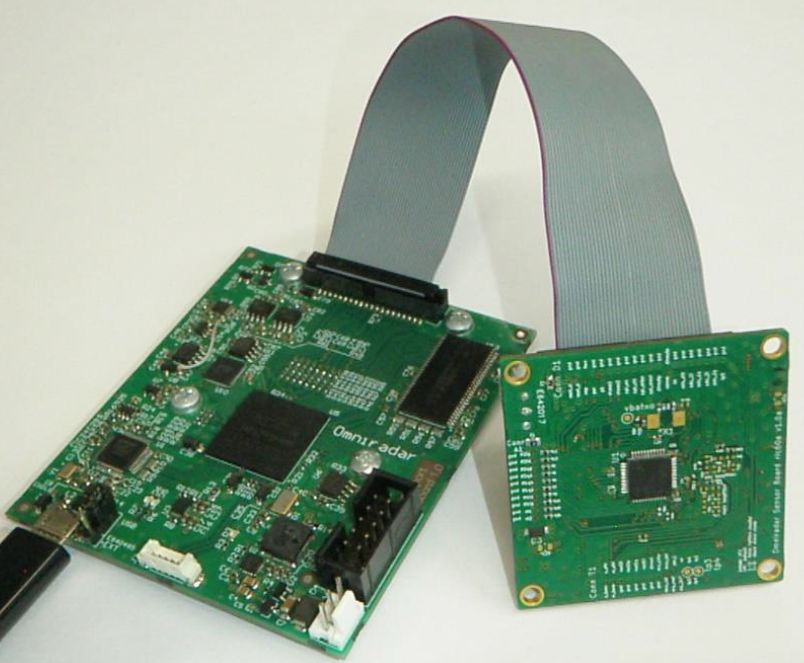
\includegraphics[width=\linewidth]{boards/img_omniradar.jpg}}$
\tabularnewline

\href{https://www.infineon.com/cms/en/product/promopages/soli/}{Google / Infineon Soli} &
Expected 2018. Sub-millimeter accuracy, running at over 10,000 frames per second \cite{Lien2016} &
\begin{minipage}[t]{\linewidth}\raggedright\strut 60~GHz\\7~GHz \strut\end{minipage} &
In\nobreakdash-package, 2~Tx,~4~Rx &
? &
$\vcenter{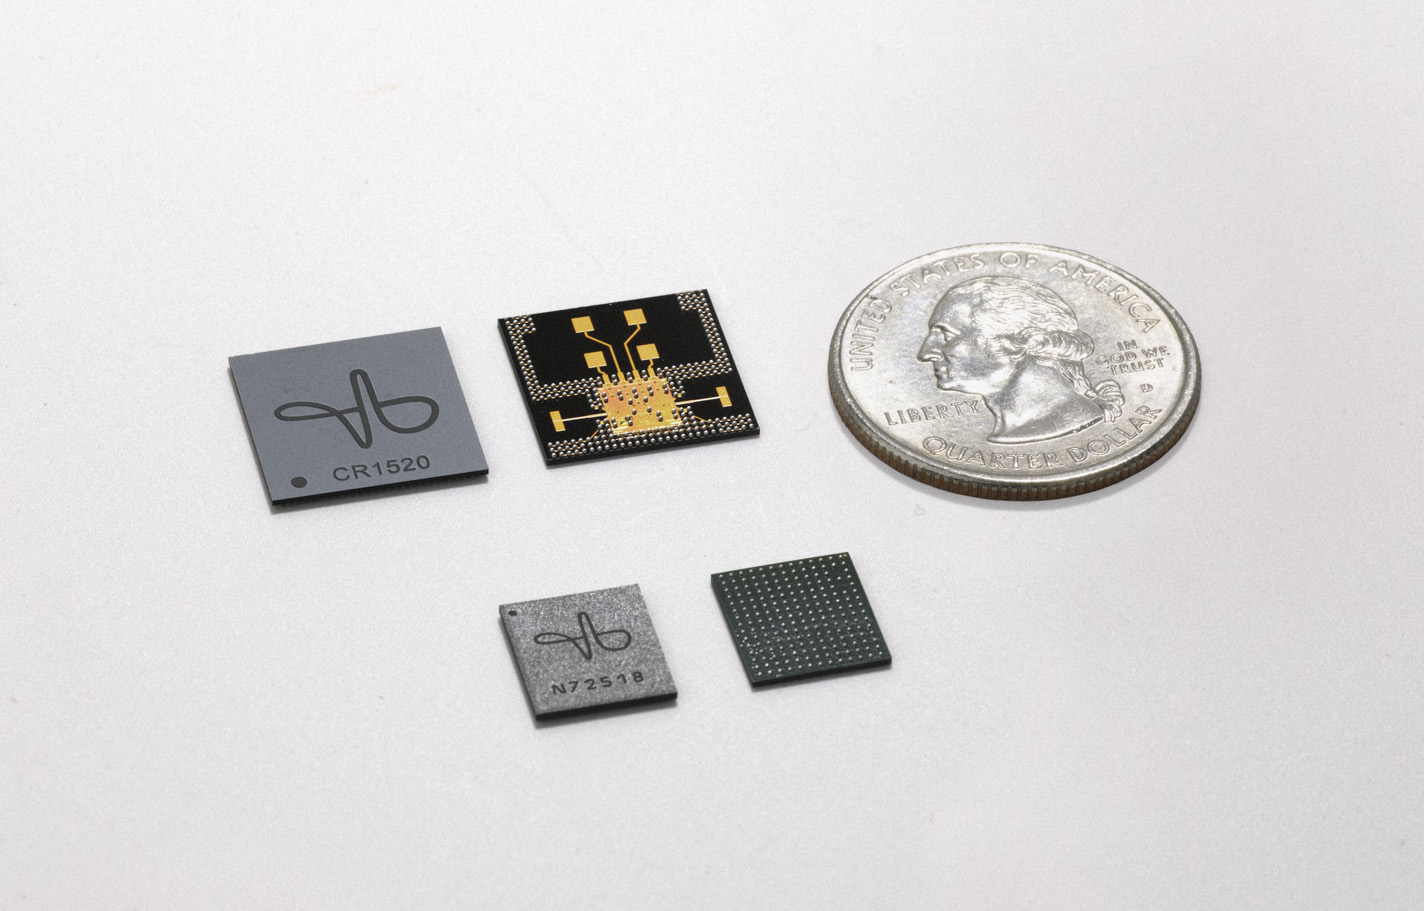
\includegraphics[width=\linewidth]{boards/img_soli.png}}$
\tabularnewline

\href{https://walabot.com/store/us/products/walabot-developer-pack.html}{Walabot Pro}&
3D configuration. Slow update rate&
\begin{minipage}[t]{\linewidth}\raggedright\strut 6.8~GHz\\7~GHz \strut\end{minipage} &
On-board, 9~Tx,~9~Rx&
\$599&
$\vcenter{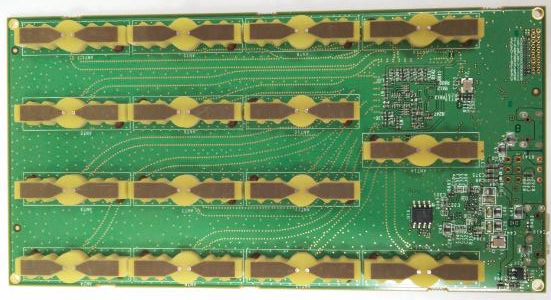
\includegraphics[width=\linewidth]{boards/img_walabot_1.png}}$
\tabularnewline

Bosch Prototype&
Prototype for In-wall pipe detection&
\begin{minipage}[t]{\linewidth}\raggedright\strut 5.15~GHz\\6.7~GHz \strut\end{minipage} &
External, 2~Tx/Rx&
\$0&
$\vcenter{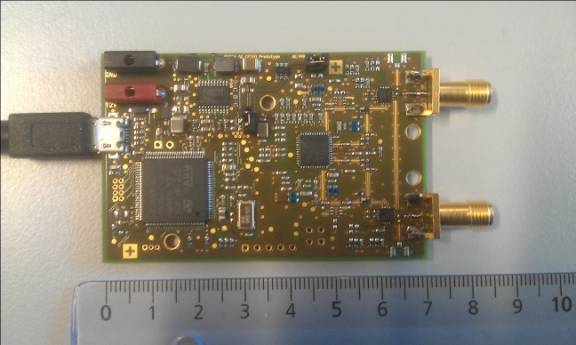
\includegraphics[width=\linewidth]{boards/img_bosch.jpg}}$
\tabularnewline

\href{http://www.siliconradar.de/evalkits_e.html}{Silicon Radar SiRad Simple}&
Has WiFi&
\begin{minipage}[t]{\linewidth}\raggedright\strut 122~GHz\\6.4~GHz \strut\end{minipage} &
On-chip, 1~Tx,~1~Rx&
?&
$\vcenter{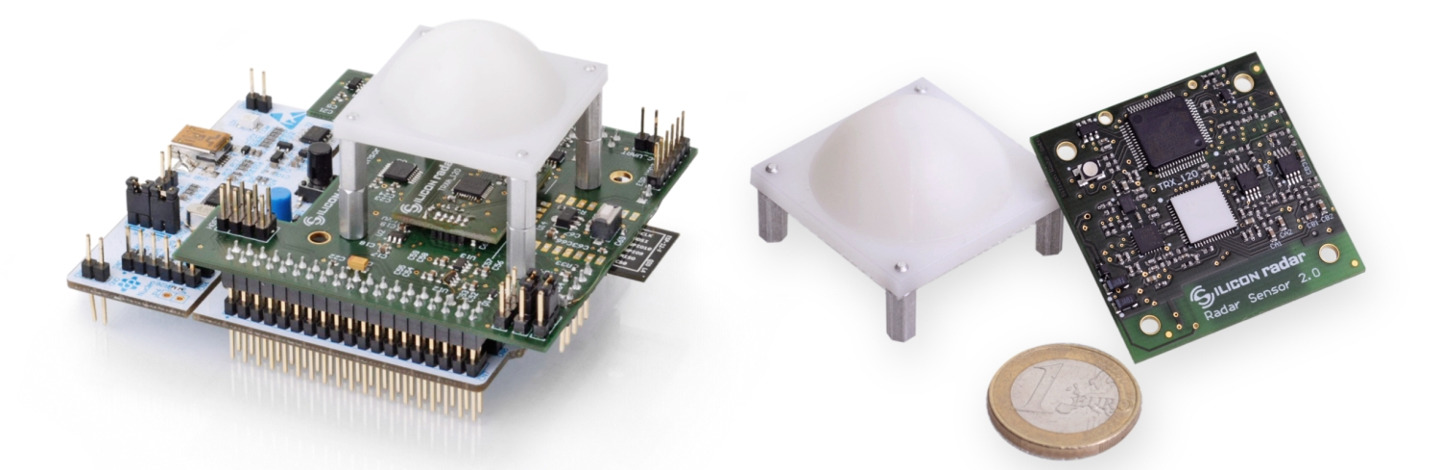
\includegraphics[width=\linewidth]{boards/img_silicon_radar.jpg}}$
\tabularnewline

\href{http://www.anokiwave.com/products/awmf-0117/index.html}{Anokiwave AWMF-0117}&
&
\begin{minipage}[t]{\linewidth}\raggedright\strut 12.5~GHz\\4.5~GHz \strut\end{minipage} &
On-chip, 1~Tx/Rx&
?&
$\vcenter{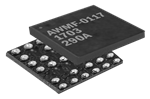
\includegraphics[width=\linewidth]{boards/img_anokiwave.png}}$
\tabularnewline

\href{Reuter2016}{NXP Cocoon Radar}&
Relatively small board. Presentation at FTF 2016\cite{Reuter2016}&
\begin{minipage}[t]{\linewidth}\raggedright\strut 77~GHz\\4~GHz \strut\end{minipage} &
On-board, 3~Tx,~4~Rx&
?&
$\vcenter{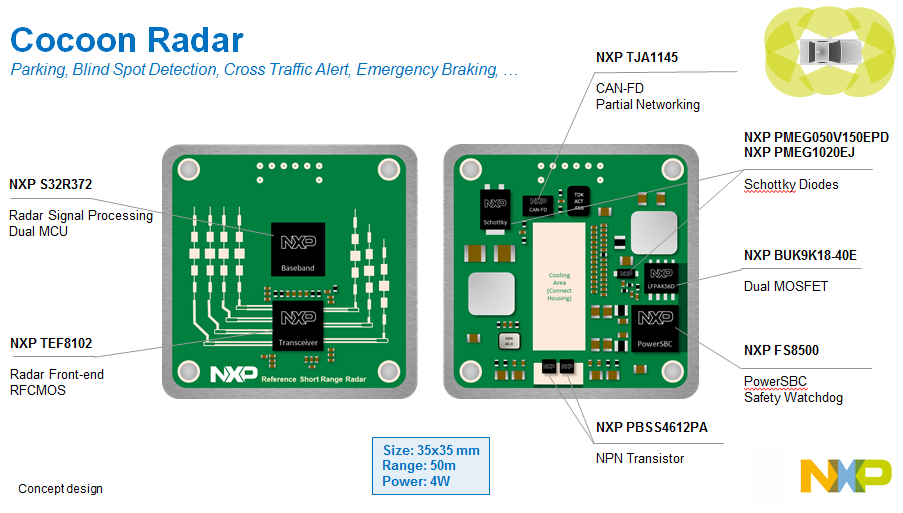
\includegraphics[width=\linewidth]{boards/img_cocoon.png}}$
\tabularnewline

\href{http://www.timedomain.com/products/pulson-440/}{TimeDomain P440}&
Can operate as multistatic radar or UWB communication node&
\begin{minipage}[t]{\linewidth}\raggedright\strut 4~GHz\\1.7~GHz \strut\end{minipage} &
External, 2~Tx/Rx&
\$5000&
$\vcenter{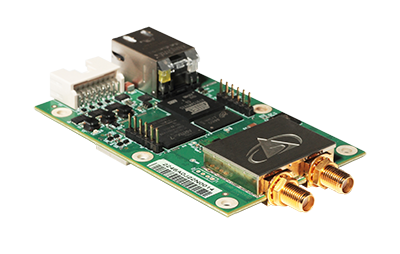
\includegraphics[width=\linewidth]{boards/img_p440.png}}$
\tabularnewline

\href{https://www.xethru.com/xethru-development-platform.html}{Novelda Xethru X4M03}&
&
\begin{minipage}[t]{\linewidth}\raggedright\strut 8~GHz\\1.5~GHz \strut\end{minipage} &
On-board, 1~Tx/Rx&
\$399&
$\vcenter{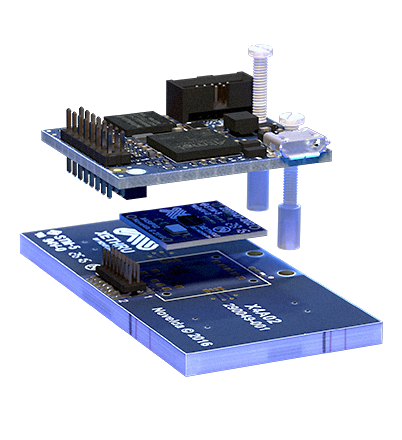
\includegraphics[width=\linewidth]{boards/img_xethru.png}}$
\tabularnewline

\href{https://www.rfbeam.ch/files/products/26/downloads/ProductBrief_MR2001_RD.pdf}{RFbeam MR2001\_RD}&
&
\begin{minipage}[t]{\linewidth}\raggedright\strut 77~GHz\\1~GHz \strut\end{minipage} &
On-board, 4~Tx,~6~Rx&
?&
$\vcenter{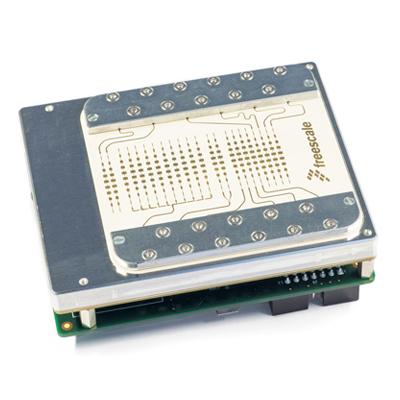
\includegraphics[width=\linewidth]{boards/img_rfbeam.jpg}}$
\tabularnewline

\href{http://www.inras.at/en/products/radarbook.html}{Inras Radarbook} (77Ghz)&
Configurable FPGA processing chain&
\begin{minipage}[t]{\linewidth}\raggedright\strut 77~GHz\\1~GHz \strut\end{minipage} &
On-board, 4~Tx,~8~Rx&
\$7300&
$\vcenter{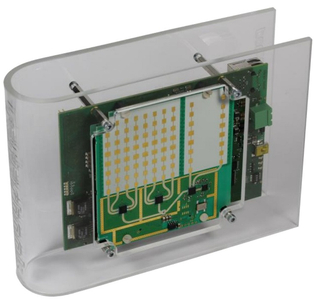
\includegraphics[width=\linewidth]{boards/img_radarbook.jpg}}$
\tabularnewline

\href{ http://www.acconeer.com/}{Acconeer A1}&
Sub-mm accuracy&
\begin{minipage}[t]{\linewidth}\raggedright\strut 60~GHz\\? \strut\end{minipage} &
On-chip, ?&
?&
$\vcenter{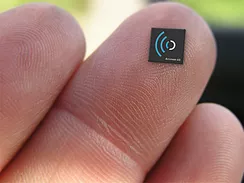
\includegraphics[width=\linewidth]{boards/img_acconeer.png}}$
\tabularnewline

\href{dkradarbook}{Inras Radarbook} (24Ghz)&
&
\begin{minipage}[t]{\linewidth}\raggedright\strut 24~GHz\\250~MHz \strut\end{minipage} &
On-board, 4~Tx,~4~Rx&
\$7300&
$\vcenter{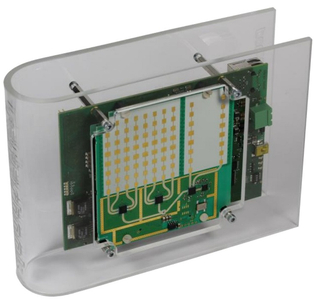
\includegraphics[width=\linewidth]{boards/img_radarbook.jpg}}$
\tabularnewline

\href{https://www.infineon.com/dgdl/Infineon-AN380_BGT24-RFB2412_user_manual-AN-v01_00-EN.pdf?fileId=5546d46259d9a4bf0159f9f1fa503f1d}{Infineon BGT24-RFB2412-EVAL}&
&
\begin{minipage}[t]{\linewidth}\raggedright\strut 24~GHz\\250~MHz \strut\end{minipage} &
On-board, 1~Tx,~2~Rx&
\$1333&
$\vcenter{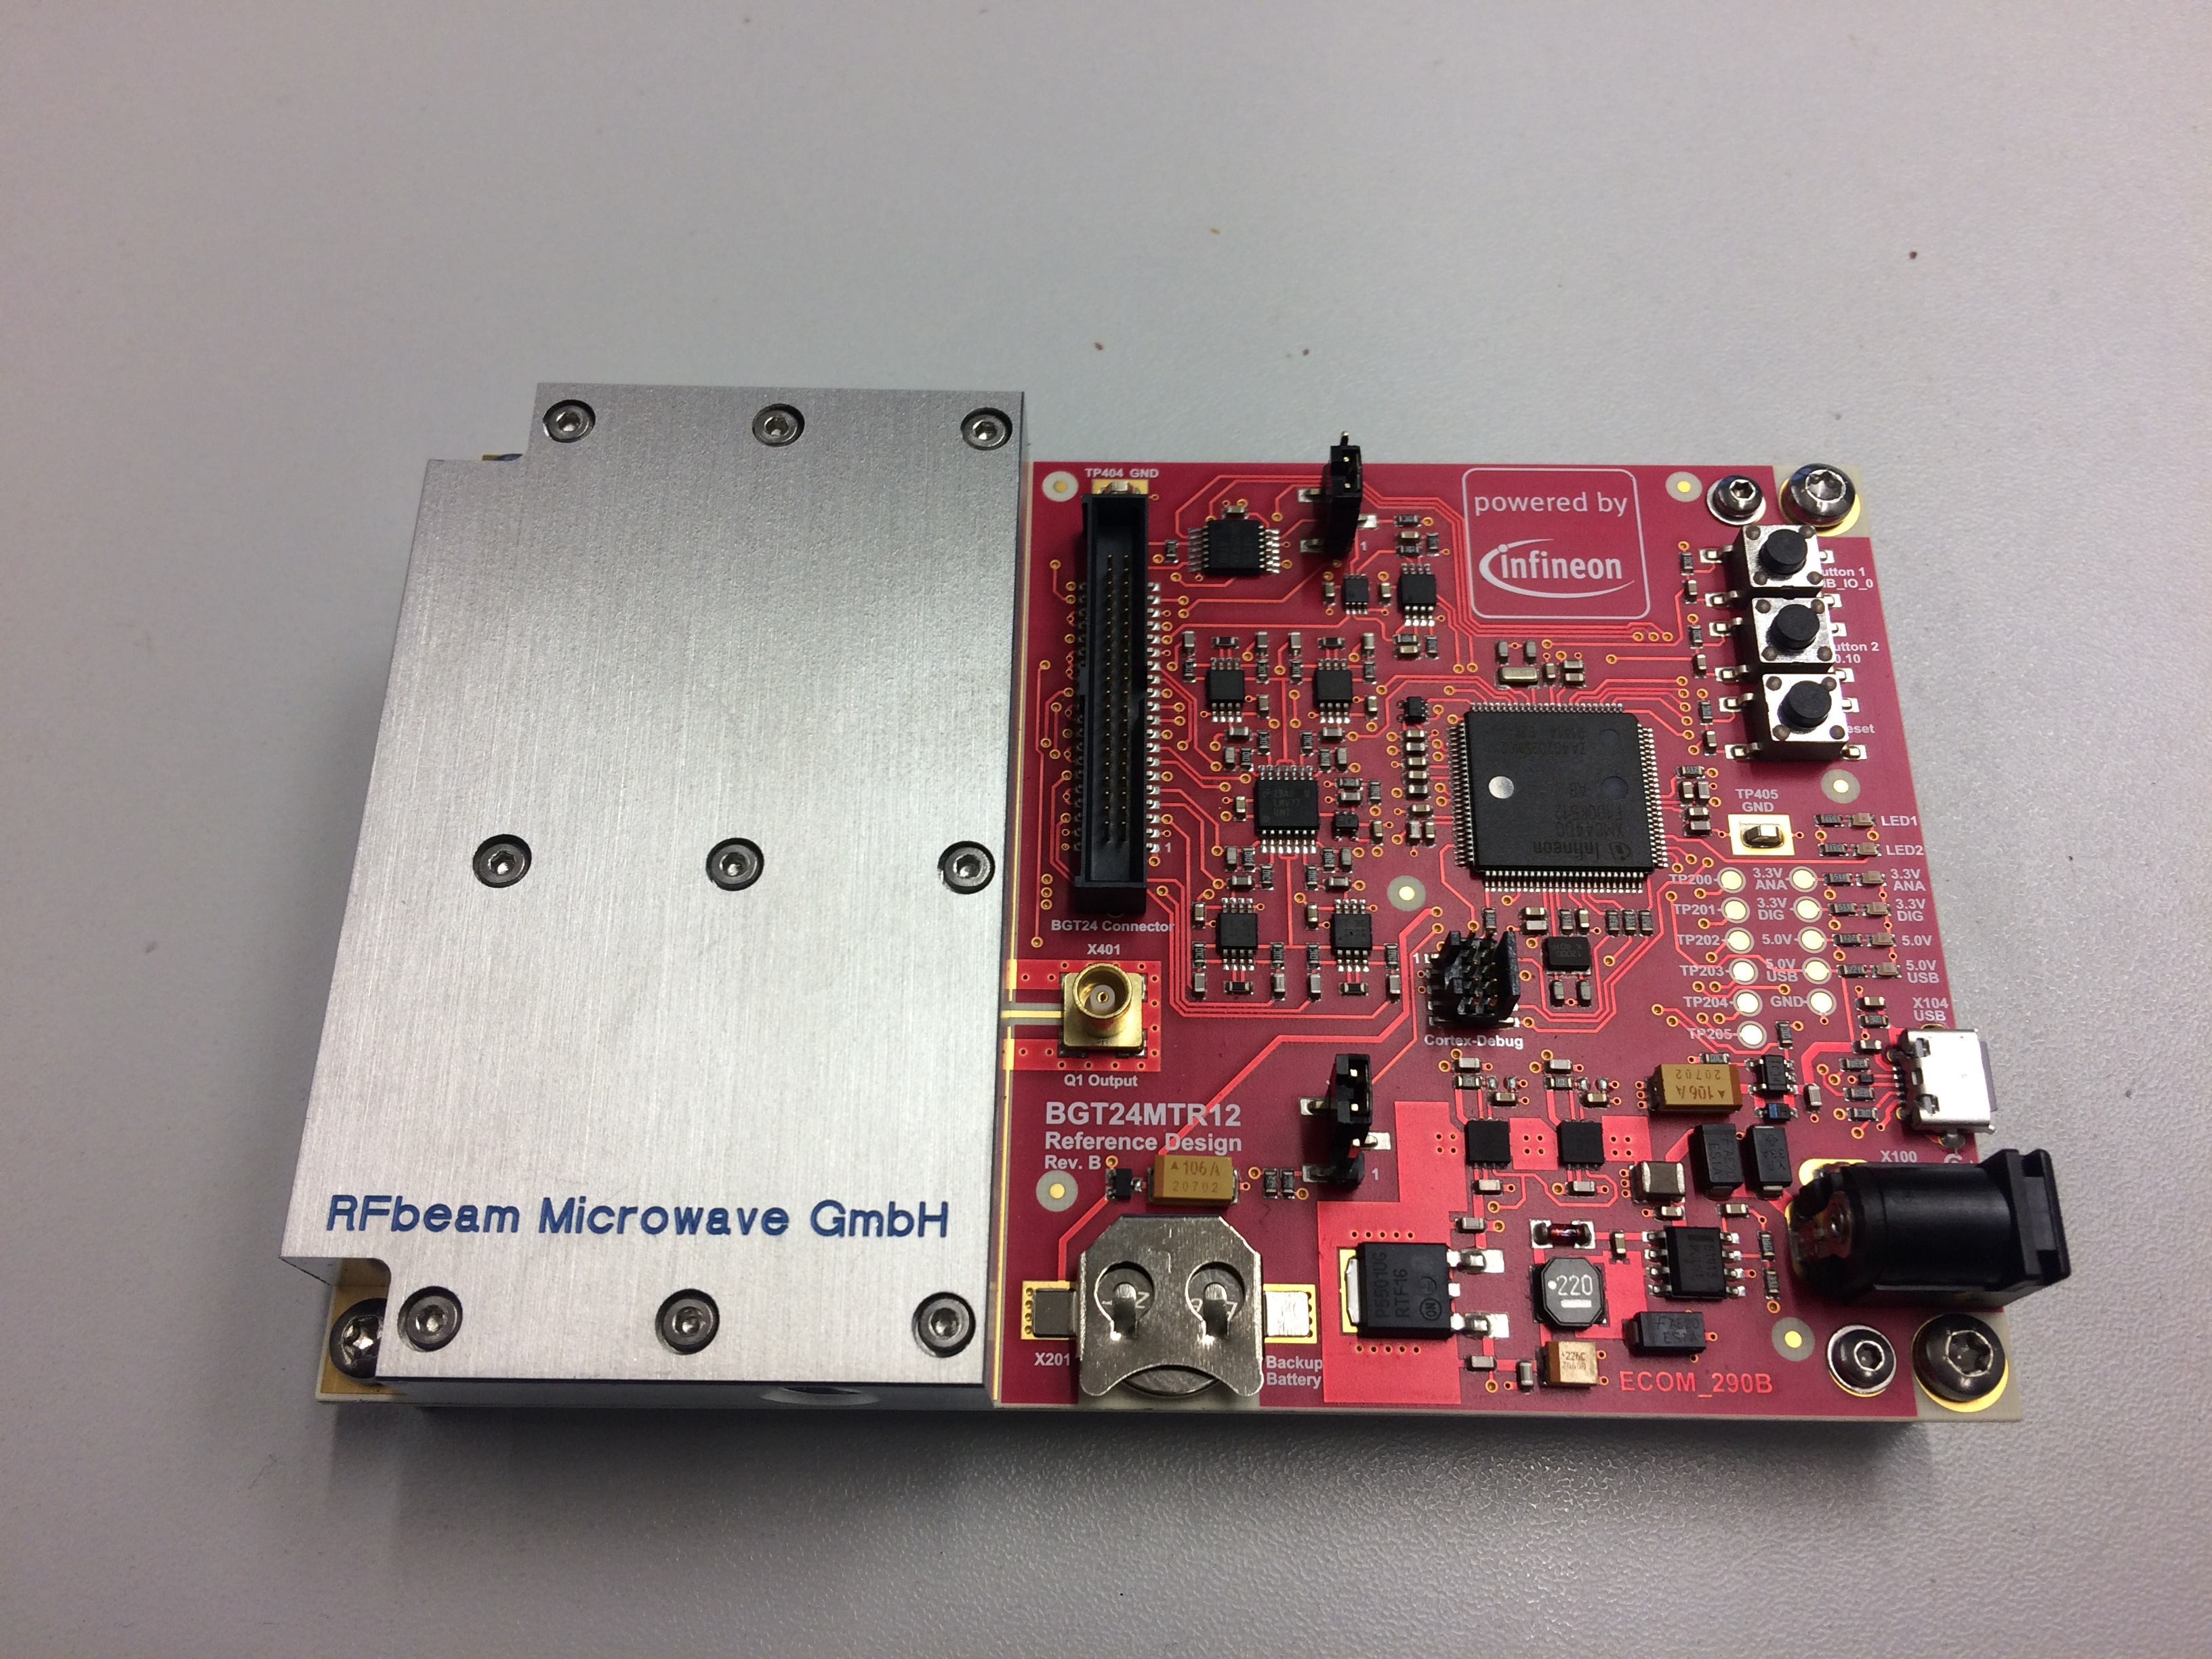
\includegraphics[width=\linewidth]{boards/img_bgt24.JPG}}$
\tabularnewline

\href{http://webshop.imst.de/dk-sr-1200e-development-platform-for-24-ghz-fmcw-radar-application.html
}{IMST DK-sR-1200e}&
&
\begin{minipage}[t]{\linewidth}\raggedright\strut 24~GHz\\250~MHz \strut\end{minipage} &
On-board, 1~Tx,~2~Rx&
\$3333&
$\vcenter{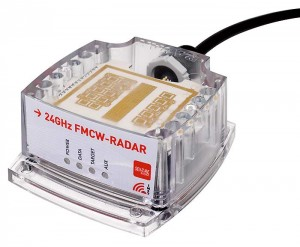
\includegraphics[width=\linewidth]{boards/img_IMST.jpg}}$
\tabularnewline

\href{http://www.innosent.de/fileadmin/media/dokumente/DATASHEETS_2016/Datenblatt_IVS-565.pdf}{InnoSenT IVS-565}&
&
\begin{minipage}[t]{\linewidth}\raggedright\strut 24~GHz\\250~MHz \strut\end{minipage} &
On-board, 1~Tx,~2~Rx&
?&
$\vcenter{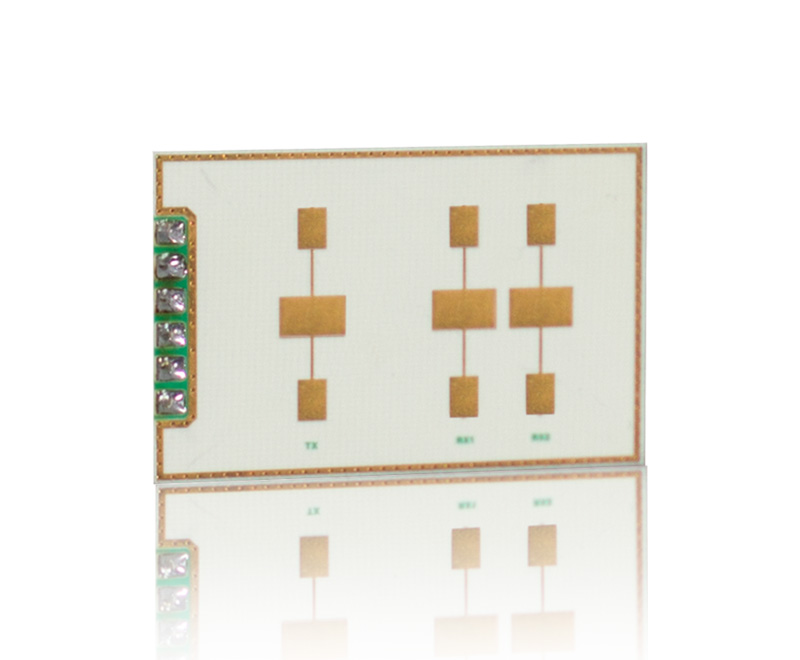
\includegraphics[width=\linewidth]{boards/img_innosent.jpg}}$
\tabularnewline

\href{http://www.st.com/content/st_com/en/products/evaluation-tools/product-evaluation-tools/automotive-ic-eval-boards/evb-strada431.html}{ST EVB-STradA431}&
SMA connectors for internal signals&
\begin{minipage}[t]{\linewidth}\raggedright\strut 24~GHz\\250~MHz \strut\end{minipage} &
External, 1~Tx,~3~Rx&
?&
$\vcenter{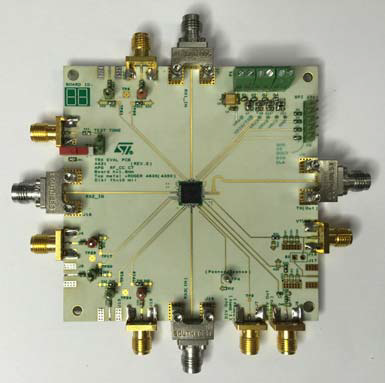
\includegraphics[width=\linewidth]{boards/img_ST.png}}$
\tabularnewline

\href{https://www.omnipresense.com/product/ops241-a/}{OmniPreSense OPS241-A}&
Arduino shield with BGT24LTR11&
\begin{minipage}[t]{\linewidth}\raggedright\strut 24~GHz\\80~MHz \strut\end{minipage} &
On-board, 1~Tx/Rx&
\$169&
$\vcenter{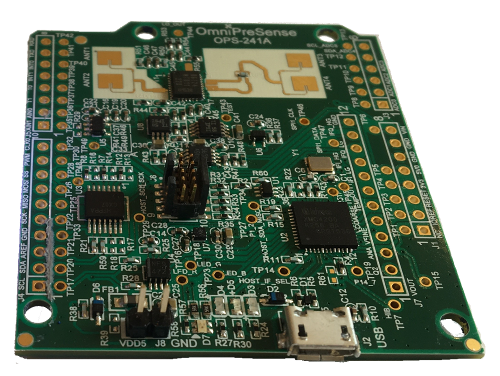
\includegraphics[width=\linewidth]{boards/img_omnipresense.png}}$
\tabularnewline


\bottomrule
\end{longtable}


